\documentclass[10pt]{nsibeamer}

\title{Chapitre 02 : Bases de données}
\subtitle{Partie 1}
\author{NSI2}

\begin{document}
	\maketitle
    \section{Introduction}
\begin{frame}{BDD et SGBD}
	Une \alert{base de données} (BDD) est un ensemble structuré de données ainsi que des relations logiques sur ces données.\\\pause

    Le \alert{système de gestion de bases de données} (SGBD) peut être vu comme le logiciel qui gère :\pause
    \begin{itemize}
    	\item	la structuration des données ;\pause
    	\item	le stockage des données ;\pause
        \item 	la maintenance des données ;\pause
        \item 	la sécurité des données ;\pause
        \item 	les accès aux données (lecture et/ou écriture) en temps réel par de multiples intervenants.
    \end{itemize}
\end{frame}

\begin{frame}{Un peu d'histoire}
	La majorité de ce que nous allons voir repose sur les travaux d'Edgar F. Codd, c'est lui qui a inventé le modèle relationnel en 1970 alors qu'il travaillait comme informaticien chez IBM.
    \begin{center}
        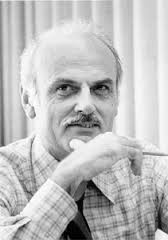
\includegraphics[width=3cm]{img/codd}
    \end{center}
\end{frame}

\begin{frame}{Phases de conception d'une BDD}
	C'est une tâche essentielle pour assurer le bon fonctionnement des applications qui vont l'utiliser.\pause
    \begin{itemize}
    	\item	\alert{niveau conceptuel} : on représente la BDD à l'aide de schémas indépendamment de toute considération informatique ;\pause
    	\item	\alert{niveau logique} on adapte le schéma en tables à deux dimensions ;\pause
        \item	\alert{niveau physique} on implémente les tables sur un SGBD.
    \end{itemize}
\end{frame}
\section{Niveau conceptuel\\ Modèle entités-associations}
\begin{frame}{Entités}
On commence par déterminer les types des entités qui interviennent:\pause
\begin{itemize}
	\item	une \alert{entité} est un objet unique avec un nombre fini d'attributs ;\pause
	\item	un (ou plusieurs) attribut(s) permet(tent) d'identifier de manière unique l'entité : on parle d'\alert{identifian}t(s) ou de clé.\pause
\end{itemize}
\begin{center}
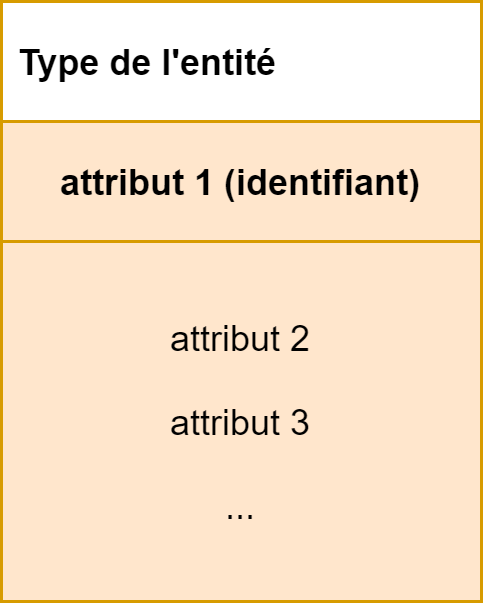
\includegraphics[width=3cm]{img/entité}
\end{center}
\end{frame}
\begin{frame}{Exemple : entité-type Auteur}
\begin{center}
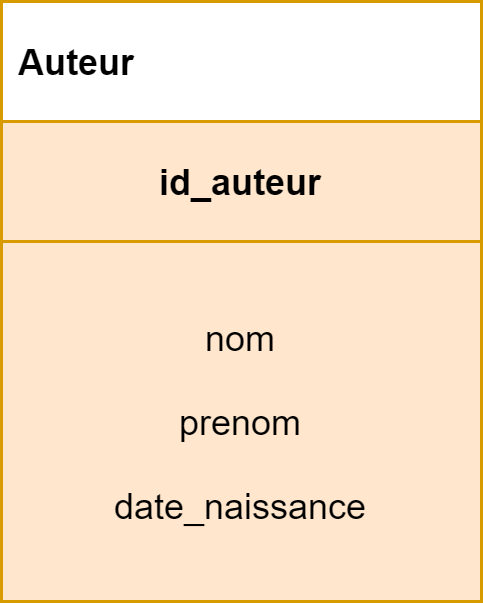
\includegraphics[width=3cm]{img/auteur}
\end{center}
\end{frame}
\begin{frame}{Occurrences}
	Une entité-type a en général plusieurs occurrences, appelées entités.\\\pause

    \begin{center}
        \begin{tabular}{cccc}
        \hline
        \rowcolor{UGLiRed!25}
        \textbf{id\_auteur }& \textbf{nom} & \textbf{prenom}&\textbf{date\_naissance}\\\hline
        \rowcolor{UGLiBlue!7}00000001 & Dupond & Marie& 23/08/1982\\
        \rowcolor{UGLiRed!7}12345678 & Martin & Luce& 13/05/1963\\
        \rowcolor{UGLiBlue!7}98765432 & Leblanc & Jean& 18/11/1974\\
         \hline
        \end{tabular}
    \end{center}\pause
    \begin{alertblock}{Remarque}
    	Par souci de simplicité, on parlera d'entité à la fois pour désigner l'entité-type et chacune de ses occurrences.
    \end{alertblock}
\end{frame}
\begin{frame}{Entité Pays}
Voici une autre entité entrant en jeu dans la BDD :
\begin{center}
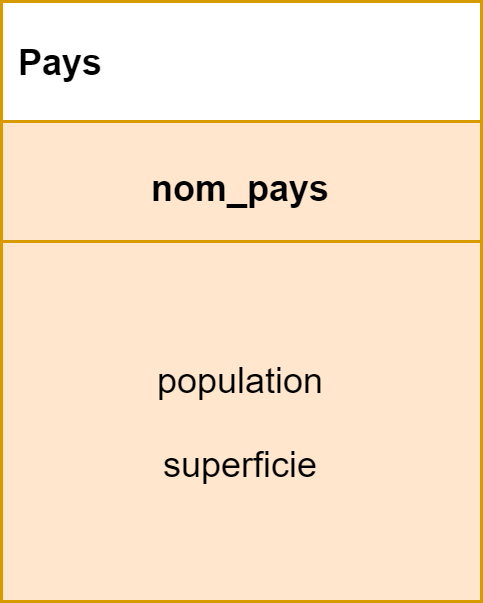
\includegraphics[width=3cm]{img/pays}
\end{center}

\end{frame}
\begin{frame}{Associations}
Elles définissent des \alert{liens sémantiques} (des liens de sens)	 que les simples entités ne suffisent pas à définir.\\\pause

Une association comporte :\pause
\begin{itemize}
	\item	un nom;\pause
    \item 	un lien entre 2 relations ;\pause
	\item	deux cardinalités qui sont représentées sur les extrémités du lien ;\pause
    \item 	parfois elle peut comporter un ou des attributs.
\end{itemize}
\end{frame}
\begin{frame}{Exemple}
	\begin{center}
    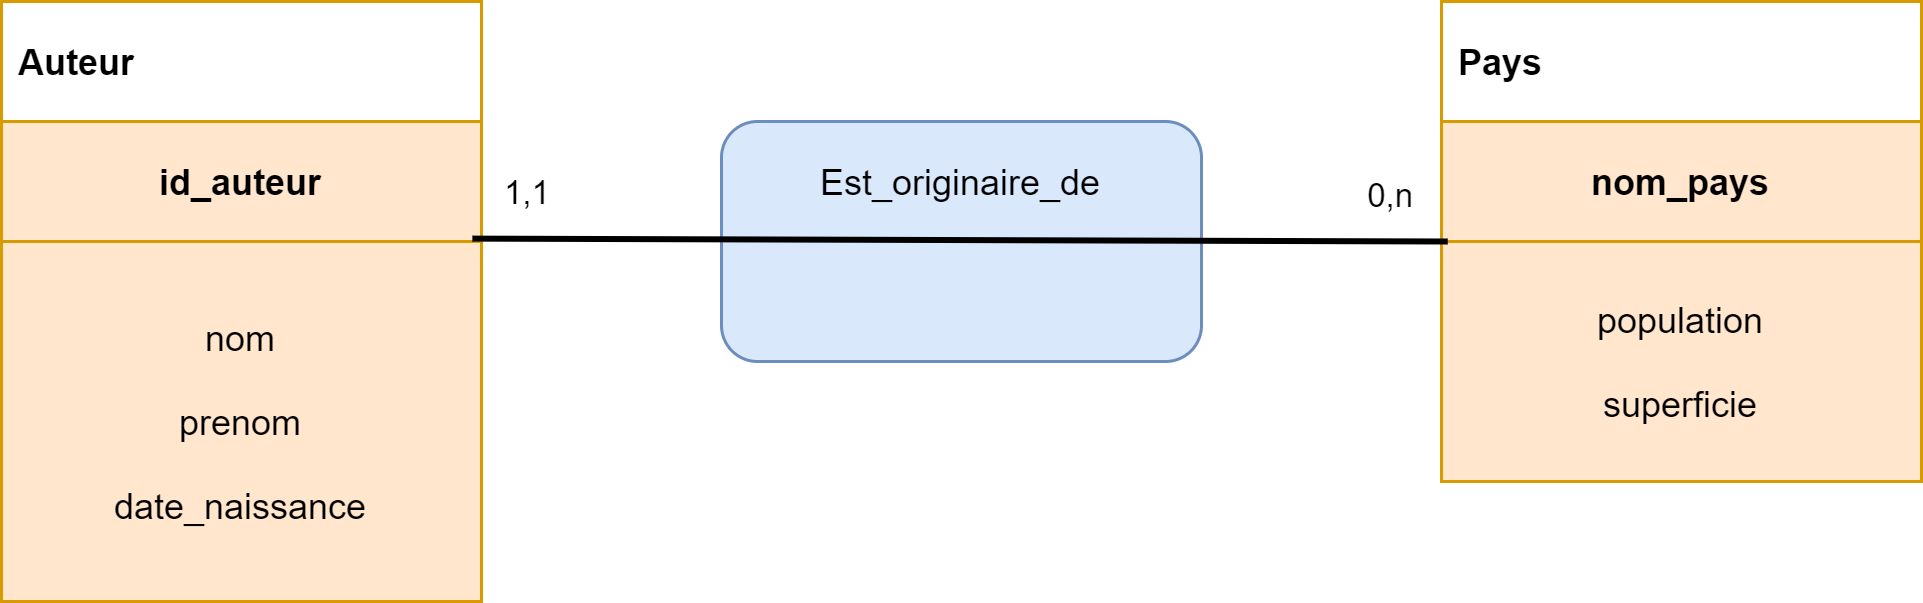
\includegraphics[width=8cm]{img/schema_1}
    \end{center}\pause
    Une cardinalité est un couple d'entiers « de type $\min, \max$» :\pause
    \begin{itemize}
    	\item	la cardinalité 1,1 signifie qu'un auteur peut être lié au minimum à 1 pays, et au maximum à 1 pays (donc à un pays et un seul) ;\pause
    	\item	la cardinalité 0,n signifie qu'un pays peut être lié au minimum à aucun auteur et au maximum plusieurs auteurs.\pause
    \end{itemize}
\end{frame}
\begin{frame}{Un schéma abouti}
\begin{center}
 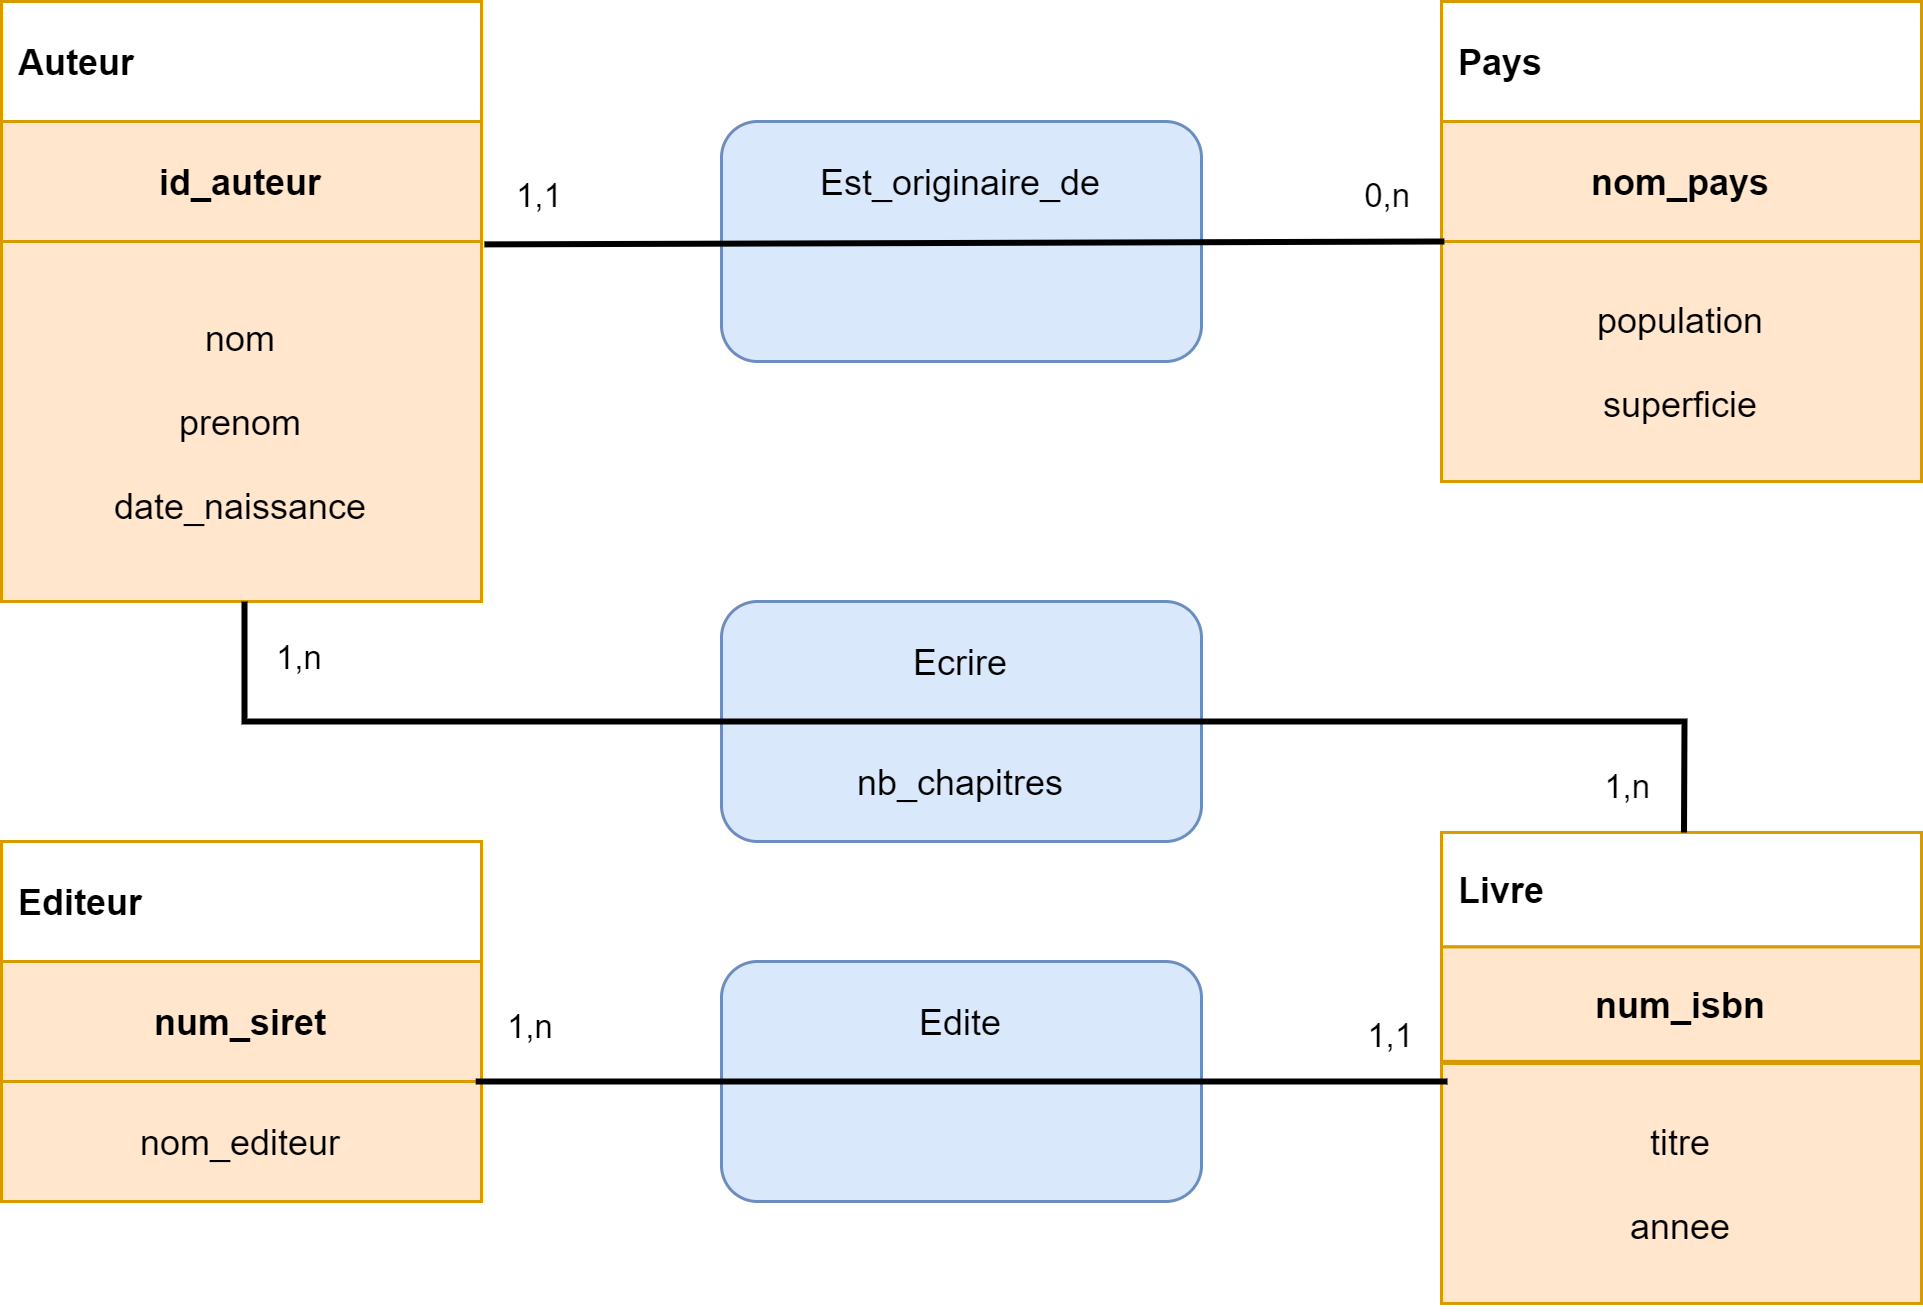
\includegraphics[width=8cm]{img/schema_2}
 \end{center}
\end{frame}
\begin{frame}{Non-unicité des schémas}
    Le schéma précédent s'appelle un modèle conceptuel des données (MCD).\\\pause
	On peut modéliser une situation avec plusieurs MCD, chacun d'entre eux ont leurs avantages et leurs inconvénients.\pause
\end{frame}
\end{document}